\textbf{5.}Considera la siguiente gram\'atica:
\[
    \begin{array}{rcl}
        E & \to & -E \mid (E) \mid VE'\\
        E' & \to & -E \mid \varepsilon\\
        V & \to & \mathtt{id}V'\\
        V' & \to & (E) \mid \varepsilon\\
    \end{array}
\]
\begin{enumerate}

    \item Muestra el c\'alculo de los conjuntos {\ffst} y {\ffollow}.

        \begin{itemize}

            \item FIRST

            \begin{itemize}

                \item FIRST(E) = \{-, (, FIRST(V)\}

                \item FIRST(E') = \{-\}

                \item FIRST(V) = \{i\}

                \item FIRST(V') = \{(\}

            \end{itemize}

            \item FOLLOW

            \begin{itemize}

                \item FOLLOW(E) = \{FIRST(E), FIRST(E')\}

                \item FOLLOW(E') = \{FIRST(E)\}

                \item FOLLOW(V) = \{d\}

                \item FOLLOW(V') = \{FIRST(E)\}

            \end{itemize}

        \end{itemize}

    \item Muestra dos \'arboles de sintaxis, uno abstracta y otro
    concreta para la cadena
    $-\mathtt{id}(-\mathtt{id})-\mathtt{id}$.

        \begin{figure}[h]
            \centering
            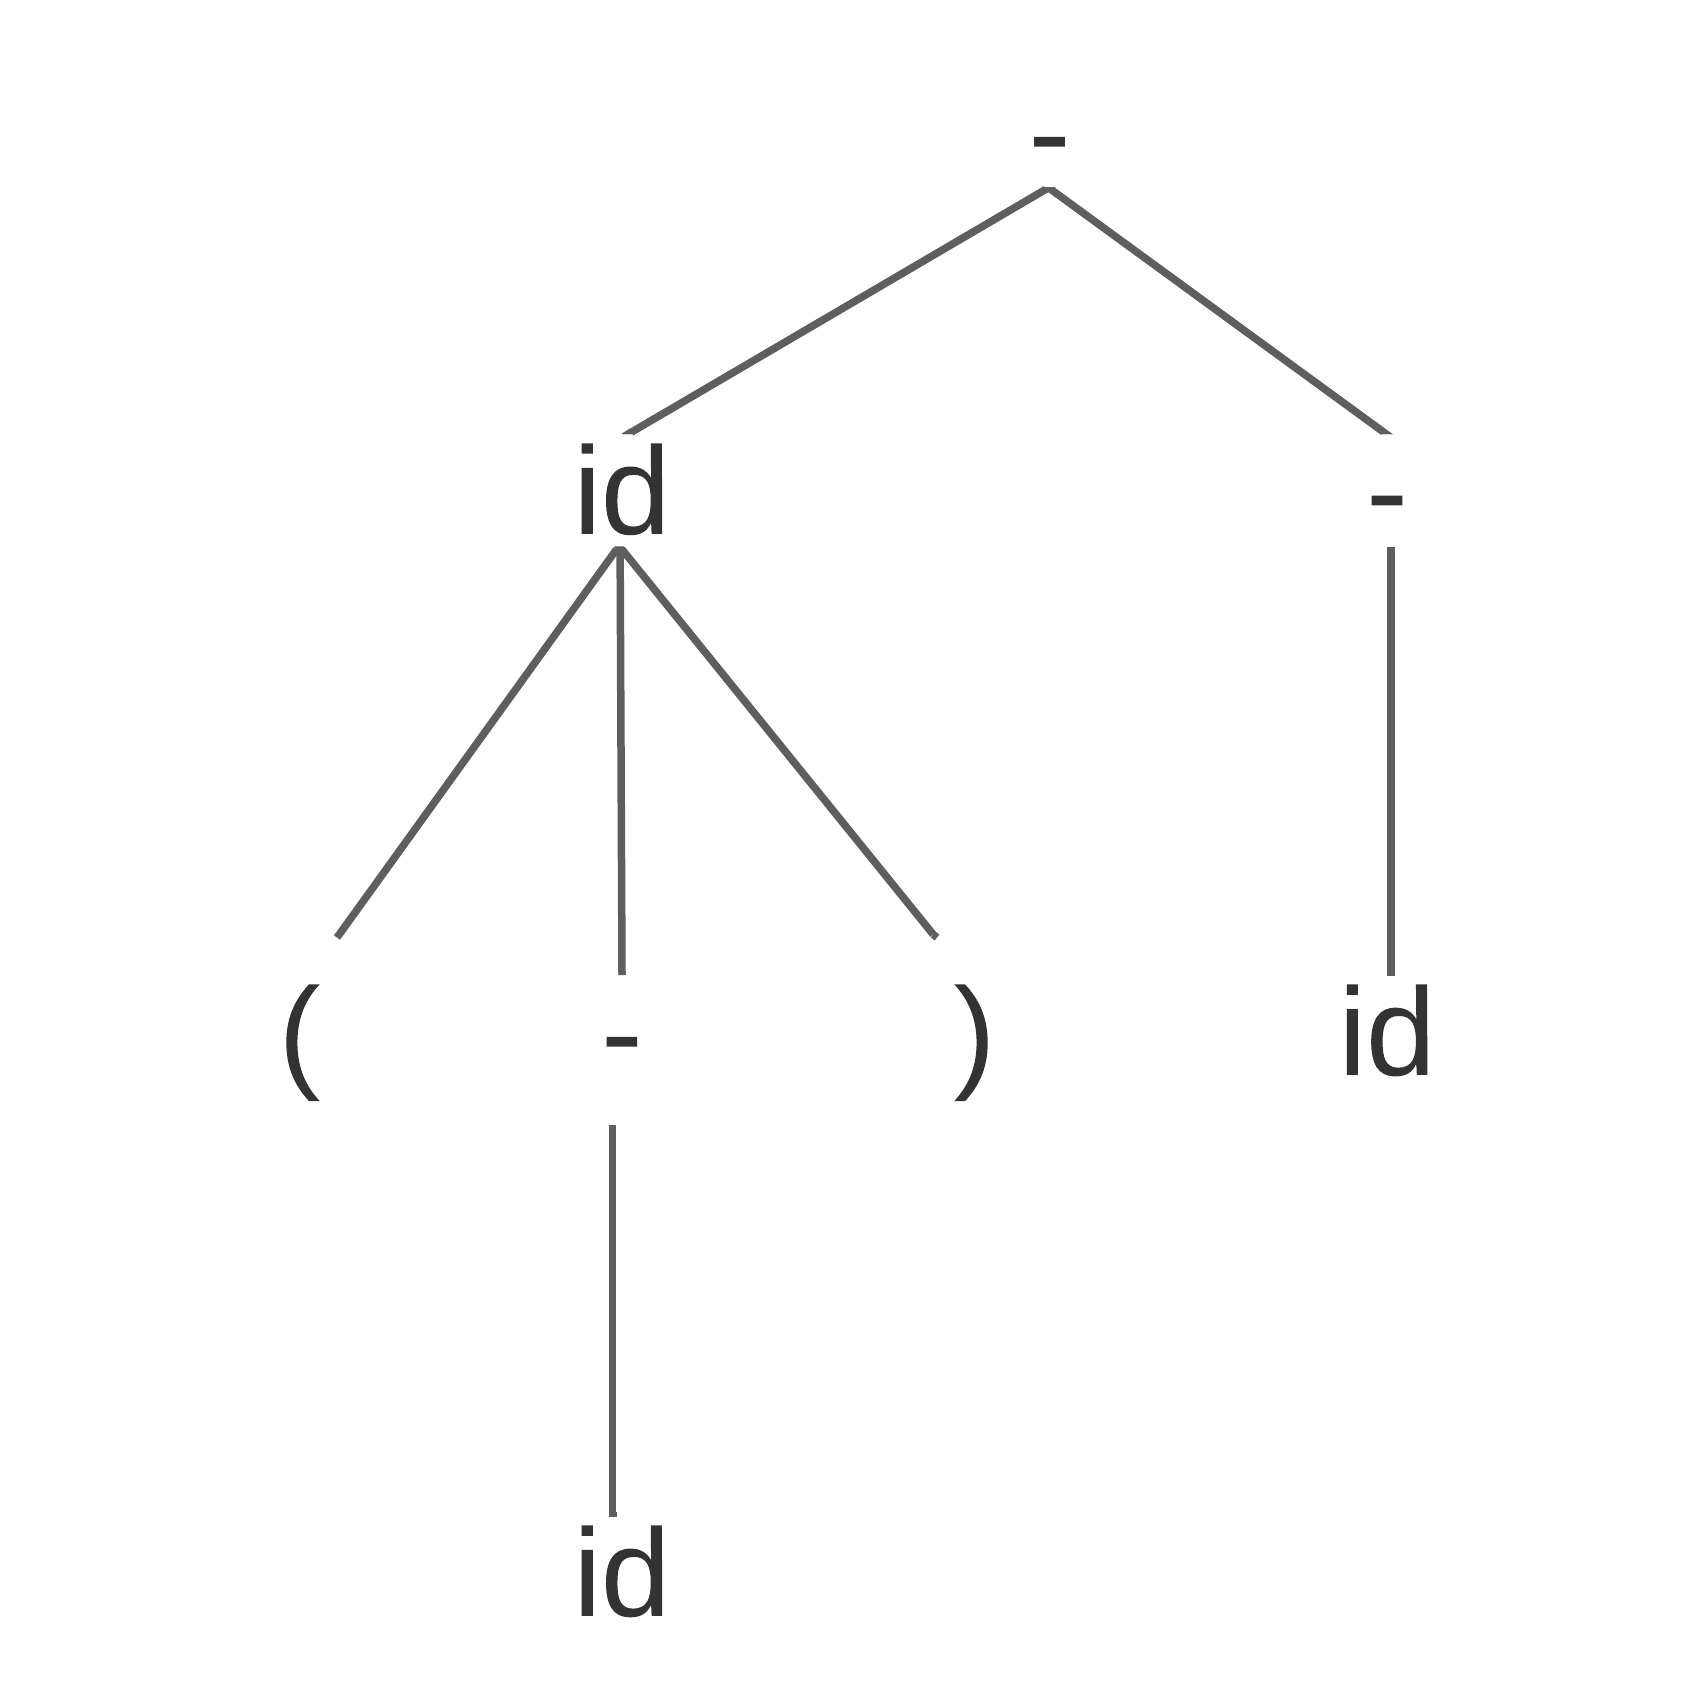
\includegraphics[scale = 0.5]{../Imagen/abst}
            \caption{Arbol de Sintaxis Abstracta}
            \label{fig:abst}
        \end{figure}

        \begin{figure}[h]
            \centering
            \includegraphics[scale = 0.5]{../Imagen/concr}
            \caption{Arbol de Sintaxis Concreta}
            \label{fig:concr}
        \end{figure}


\end{enumerate}